\documentclass[manuscript,review,anonymous,nonacm,screen]{acmart}
\usepackage{graphicx}\graphicspath{{../figures/}}
\usepackage{array}\usepackage{colortbl}\usepackage{longtable}\usepackage{subcaption}\usepackage{enumitem}
\definecolor{g}{RGB}{26,152,80}\definecolor{a}{RGB}{254,224,139}\definecolor{r}{RGB}{215,48,39}
\newcommand{\PROVIDER}{an institutional vLLM API}
\newcommand{\REPO}{a public repository (URL omitted for anonymous review)}
\newcommand{\corpustabref}{the released corpus}
\newcommand{\sttwotabref}{Table~\ref{tab:study2full}}
% auto-generated - do not edit by hand (see analysis/make_figures.py)
\newcommand{\Nstudies}{217}
\newcommand{\Ndomains}{29}
\newcommand{\Nvalidated}{8}
\newcommand{\Npromising}{60}
\newcommand{\Nmixed}{108}
\newcommand{\Ncaution}{39}
\newcommand{\Nunreliable}{2}
\newcommand{\Pctreliable}{31}
\newcommand{\Pctproblematic}{19}
\newcommand{\Nnumeric}{29}
\newcommand{\Nprimary}{206}
\newcommand{\Nsecondary}{11}
\newcommand{\Ngreen}{8}
\newcommand{\Namber}{19}
\newcommand{\Nred}{2}
\newcommand{\OAretrieved}{1500}
\newcommand{\OAunique}{957}
\newcommand{\OAtopical}{165}
\newcommand{\Webhits}{472}
\newcommand{\Webunique}{304}
\newcommand{\Nassessed}{263}
\newcommand{\Nexclscreen}{967}
\newcommand{\Crossdup}{31}
\newcommand{\Meanrel}{3.15}
\newcommand{\Nparity}{15}
% auto-generated
\newcommand{\STN}{55}
\newcommand{\STaugment}{36}
\newcommand{\STreplace}{14}
\newcommand{\STsimulate}{5}
\newcommand{\STtension}{38}
\newcommand{\STcritical}{8}
\newcommand{\STenabling}{9}
\newcommand{\SThci}{22}
\newcommand{\STmethods}{15}
\newcommand{\STrelaugment}{3.17}
\newcommand{\STrelreplace}{3.07}
\newcommand{\STrelsim}{2.8}
\newcommand{\STincluded}{55}
\newcommand{\SToa}{857}
% auto-generated
\newcommand{\STHRn}{15000}
\newcommand{\STHRdatasets}{5}
\newcommand{\STHRmodels}{6}
\newcommand{\STHRpass}{6}

% auto-generated by results_table1b.py
\newcommand{\ONEmodels}{4}
\newcommand{\ONEpanel}{\texttt{deepseek-v4-pro}, \texttt{glm-5.1}, \texttt{gptoss-120b}, \texttt{qwen3.6-35b-a3b}}
\newcommand{\ONEnjudg}{25,600}
\newcommand{\ONEbest}{\texttt{deepseek-v4-pro}}
\newcommand{\ONEbestrho}{0.542}
\newcommand{\ONEreportedrho}{0.52}
\newcommand{\ONEbeataspects}{1}
\newcommand{\ONEnsurpass}{3}
\newcommand{\ONEverdictphrase}{The most powerful open models now \emph{match or exceed} the reported proprietary-judge correlations on SummEval.}
% auto-generated by mixed_effects.py
\newcommand{\SMEsubjOR}{0.21}
\newcommand{\SMEsubjP}{6e-6}
\newcommand{\SMEsizeOR}{1.22}
\newcommand{\SMEsizeP}{0.000}
\newcommand{\SMEsizeZ}{9.63}
\newcommand{\SMEfdrtests}{30}
\newcommand{\SMEfdrsig}{25}
\newcommand{\SMEfdrbelow}{20}
\newcommand{\SMEfdrabove}{5}
\newcommand{\SMEvcdataset}{0.83}
\newcommand{\SMEvcitem}{2.21}
\newcommand{\SMEglmmsubj}{-0.57}
\newcommand{\SMEglmmsize}{0.37}
% auto-generated by make_revision_macros.py
\newcommand{\IRRsoneA}{0.87}
\newcommand{\IRRsoneWone}{100}
\newcommand{\IRRsoneEx}{74}
\newcommand{\IRRsoneN}{54}
\newcommand{\IRRstwoV}{0.85}
\newcommand{\IRRstwoRole}{0.80}
\newcommand{\IRRstwoStance}{0.59}
\newcommand{\IRRstwoN}{16}
\newcommand{\GLMsubjOR}{0.74}
\newcommand{\GLMsubjP}{0.45}
\newcommand{\GLMbaseOR}{8.2}
\newcommand{\GLMbaseP}{<.001}
\newcommand{\GLMsizeOR}{1.30}
\newcommand{\GLMsizeP}{<.001}
\newcommand{\GLMgranOR}{0.84}
\newcommand{\GLMgranP}{0.02}
\newcommand{\VCitem}{2.02}
\newcommand{\VCdataset}{0.73}
\newcommand{\VCmodel}{0.086}
\newcommand{\metaSlope}{-0.39}
\newcommand{\metaLODOmin}{-0.57}
\newcommand{\metaLODOmax}{-0.01}
\newcommand{\metaN}{6}
\newcommand{\SEfluSD}{0.63}
\newcommand{\SEconSD}{0.81}
\newcommand{\SEfluTop}{80}
\newcommand{\SEfluSelf}{0.87}
\newcommand{\MPCgenderGap}{0.01}
\newcommand{\CCmaxOverlap}{0.45}
\newcommand{\CCflag}{MEDIUM}
\newcommand{\PRstable}{10}
\newcommand{\PRtotal}{18}
\newcommand{\PRmaxSD}{0.14}
\newcommand{\PRmeanSD}{0.03}

% auto-generated by rev2_analysis.py
\newcommand{\RTwobeats}{5}
\newcommand{\RTwosubjOR}{0.98}
\newcommand{\RTwosubjP}{0.45}
\newcommand{\RTwobaseOR}{1.28}
\newcommand{\RTwosizeOR}{1.21}
\newcommand{\RTwometaCIlo}{-1.74}
\newcommand{\RTwometaCIhi}{1.66}
\newcommand{\RTwoablCeilThree}{0.81}
\newcommand{\RTwoablWRThree}{0.88}
\newcommand{\RTwoablCeilFull}{0.75}
% auto-generated by split_tables.py
\newcommand{\NLInjudg}{6,000}
\newcommand{\NLIndat}{2}
\newcommand{\NLIlowH}{0.79}
\newcommand{\NLIhighH}{0.61}
\newcommand{\SOCnjudg}{12,000}
\newcommand{\SOCndat}{4}
\newcommand{\SOClowH}{0.73}
\newcommand{\SOChighH}{0.54}

\begin{document}
\title{Augment, Replace, or Simulate? A Systematic Review and Empirical Evaluation of LLMs as Substitutes for Human Input in Human-Centered Computing}
\author{Anonymous Author(s)}
\affiliation{\institution{Anonymous Institution}\country{}}
\renewcommand{\shortauthors}{Anonymous Author(s)}
\begin{abstract}\noindent
Human-Centered Computing (HCC) research increasingly uses large language models to stand in for human input: to
code qualitative data, annotate crowdsourced corpora, simulate study participants, and generate personas. This
raises an epistemological question for a field built on interpretation, reflexivity, and situated knowledge: when
can an LLM substitute for a human, and when must a human remain in the loop? We answer with a review paired with a
new experiment. \textbf{Study 1} is a PRISMA systematic review of \STN{} HCC, HCI, and qualitative-methods studies
(all references independently web-verified), coding each on method, the LLM's intended role
(augment / replace / simulate), the reported reliability against a human baseline, and the epistemic stance. The
field overwhelmingly positions LLMs to \emph{augment} rather than replace humans (\STaugment{} augment vs.\
\STreplace{} replace vs.\ \STsimulate{} simulate), under a stance dominated by \emph{tension}, with reliability
ordered augment $>$ replace $>$ simulate. \textbf{Study 2} tests the field's central boundary empirically: we run a
six-model open panel (9B-754B) as virtual annotators on \SOCndat{} subjective social-computing datasets that carry
human label distributions (emotion, offensiveness, hate, irony; \SOCnjudg{} judgments), benchmarked against the
human-human agreement ceiling with chance-corrected agreement, a calibrated contamination screen, and an item-level
mixed-effects analysis. The augment-not-replace consensus is empirically warranted: open judges fall short of the
human ceiling on every subjective construct, and, tellingly, the judge-vs-ceiling gap is \emph{largest where humans
most agree} ($\SOCgapLow$ on low-disagreement items), so the shortfall is a genuine substitution failure, not a
label-noise artifact on ambiguous cases. Residual variance is item-level ($\mathrm{SD}_{\text{logit}}=
\SOCitemSDlogit$ vs model $\SOCmodelSDlogit$), not model scale or contamination, which we confirm on a recent
post-cutoff corpus. We translate this into an evidence-based decision framework for when HCC researchers should
automate, augment with a human in the loop, or keep humans.
\end{abstract}
\keywords{human-centered computing, LLM substitution, qualitative coding, crowdsourced annotation, participant simulation, human-AI collaboration, annotator disagreement}
\maketitle
% =====================================================================
\section{Introduction}
% =====================================================================
In barely two years, large language models have moved from objects of HCI study to \emph{instruments} of HCI method.
Researchers now use them to code interview transcripts \citep{xiao2023support,gao2024collabcoder}, run thematic
analyses \citep{depaoli2023inductive,dai2023llminloop}, annotate social-media corpora
\citep{gilardi2023chatgpt,tornberg2023political}, simulate survey respondents \citep{argyle2023outofone}, and
generate personas \citep{salminen2024deusexmachina}. The appeal is obvious: human judgment is the costly bottleneck
of human-centered research. The danger is equally clear. HCC and qualitative methods are not mere labeling
pipelines; they carry epistemological commitments, interpretation, reflexivity, positionality, and situated
knowledge, that an LLM cannot obviously honor \citep{schroeder2025usestensions,davison2024ethics}, and substituting
a model for a human participant can flatten the very identity groups HCI seeks to center
\citep{wang2024flatten,cheng2023compost}.

The field therefore faces a question with no consolidated answer: \textbf{for which HCC tasks is an LLM a safe
substitute for human input, for which is it a useful assistant, and for which is it unsafe?} We answer with two
complementary studies. First, a systematic review of how HCC \emph{actually} uses LLMs and how reliable that use is.
Second, because a review alone cannot settle a contested empirical boundary (and because the field rightly distrusts
AI-generated literature surveys without new evidence), we run a controlled experiment on the field's central case:
subjective social-computing annotation, the kind of labeling HCC and CSCW depend on for studies of affect,
toxicity, and online behavior. Throughout, we measure LLMs against the \emph{human-human agreement ceiling} computed
from each dataset's own annotators, because for subjective constructs there is no single ground truth
\citep{aroyo2015truth,plank2022humanlabel}, and we use \emph{open, locally-servable} models, the realistic choice
for most HCC labs.

\paragraph{Contributions.} (1) \textbf{Study 1:} the first systematic review (PRISMA, \STN{} studies, all references
web-verified) of LLM substitution specifically for HCC/HCI/qualitative methods, coding method $\times$ role
(augment/replace/simulate) $\times$ epistemic stance, which surfaces an augment-not-replace consensus and its
tensions. (2) \textbf{Study 2:} a new empirical evaluation of a six-model open panel on \SOCndat{} subjective
social-computing datasets with human label distributions (\SOCnjudg{} judgments), showing the consensus is
empirically warranted and that item-level human disagreement, not model scale, governs reliability. (3) An
evidence-based decision framework for HCC practice. All code, corpora, and harnesses are released.
\section{Study 1: LLM substitution in HCC, HCI, and qualitative methods}
% =====================================================================
\subsection{Motivation and research questions}
Cross-domain evidence (our companion paper) shows LLM-judge reliability is broadly domain-general; HCC needs a method-specific account. Human-centered research is built on methods
that historically \emph{require} human input: qualitative coding, thematic and content analysis, interviews and
open-ended survey analysis, crowdsourced annotation, participant studies, persona development, usability/heuristic
evaluation, and design critique. Study 1 asks: \textbf{(RQ1.1)} which of these methods have been attempted with
LLMs, and how reliably do LLM outputs agree with human input? \textbf{(RQ1.2)} How does the field position the
LLM, to \emph{augment}, \emph{replace}, or \emph{simulate} the human? \textbf{(RQ1.3)} What epistemic stance
(enabling, tension, critical) does the literature take, and what does that imply for HCC practice?

\subsection{Method}
Following the shared protocol, we ran a Study-2-specific identification arm: 25 HCC/HCI/qualitative concept-block
queries against OpenAlex (\SToa{} unique works), triangulated with the web arm and a venue-scoped sweep of HCI venues (CHI, CSCW, UIST, IUI, TOCHI). After topicality screening and eligibility assessment we included
\STN{} studies (Figure~\ref{fig:s2prisma}). An independent re-coding of a 30\% sample ($n{=}\IRRstwoN$) reproduced
the verdict at Krippendorff $\alpha=\IRRstwoV$ and the augment/replace/simulate role at $\alpha=\IRRstwoRole$; the
\emph{epistemic stance} code is the least reliable ($\alpha=\IRRstwoStance$), so we treat stance-based claims as
indicative rather than precise (Appendix~\ref{app:irr}). We extracted, per study: the HCC \textbf{method}; the LLM \textbf{role}
(replace / augment / simulate); reported agreement and the human baseline; the reliability \textbf{verdict};
the \textbf{epistemic stance} (enabling / tension / critical); and the \textbf{community} (HCI, CSCW,
qualitative-methods, computational social science, NLP, health). The full corpus is \sttwotabref.

\begin{figure}[t]\centering
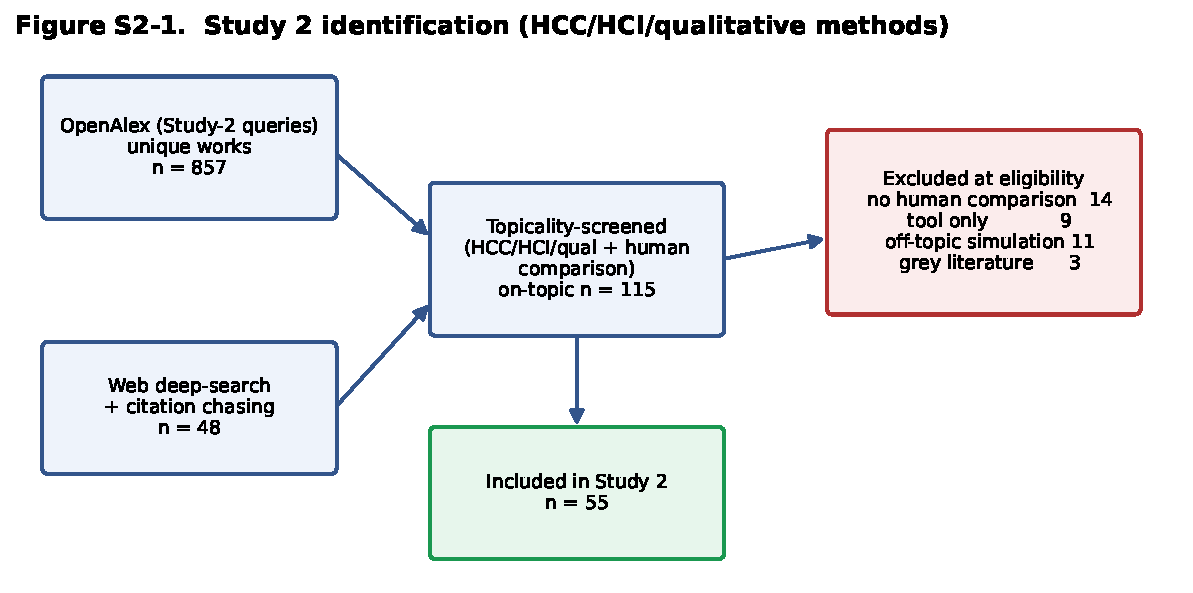
\includegraphics[width=0.96\linewidth]{s2_fig01_prisma}
\caption{Study 1 identification flow (HCC/HCI/qualitative methods).}
\label{fig:s2prisma}
\end{figure}

\subsection{RQ1.1: Which methods, and how reliable?}
LLMs have been compared against human input across \STmethods{} distinct HCC methods
(Figure~\ref{fig:s2methods}), most heavily in \emph{thematic analysis}, \emph{synthetic participants}, and
\emph{crowdsourced annotation}. Reliability is strongly method-dependent (Figure~\ref{fig:s2relmethod};
Table~\ref{tab:s2methods}). The \emph{same objectivity/interpretation axis} seen across domains governs HCC:
\textbf{objective crowd-annotation} is the most reliable method to substitute: ChatGPT matches or beats crowd
workers and even trained coders on stance, topic, and frame labeling \citep{gilardi2023chatgpt,tornberg2023political};
\textbf{deductive/inductive coding and content/thematic analysis} are reliable \emph{as augmentation}, with
human-equivalent agreement on structured codebooks (GPT-4 exceeding substantial $\kappa$ on 8/9 hermeneutic tasks
\citep{dunivin2024scalablecot}; Gemini $\kappa=0.907$ in multi-LLM thematic analysis \citep{jain2025multillmthematic};
79.7\% agreement in health thematic summarization \citep{castellanos2025thematicsumm}) but only moderate agreement
in open interpretive settings ($\kappa\approx0.40$-$0.46$ \citep{li2024gpt4humanqual,qualcoding2025jla}); and
\textbf{participant/persona simulation and usability evaluation} are the least reliable.

\begin{figure}[t]\centering
\begin{subfigure}{0.52\linewidth}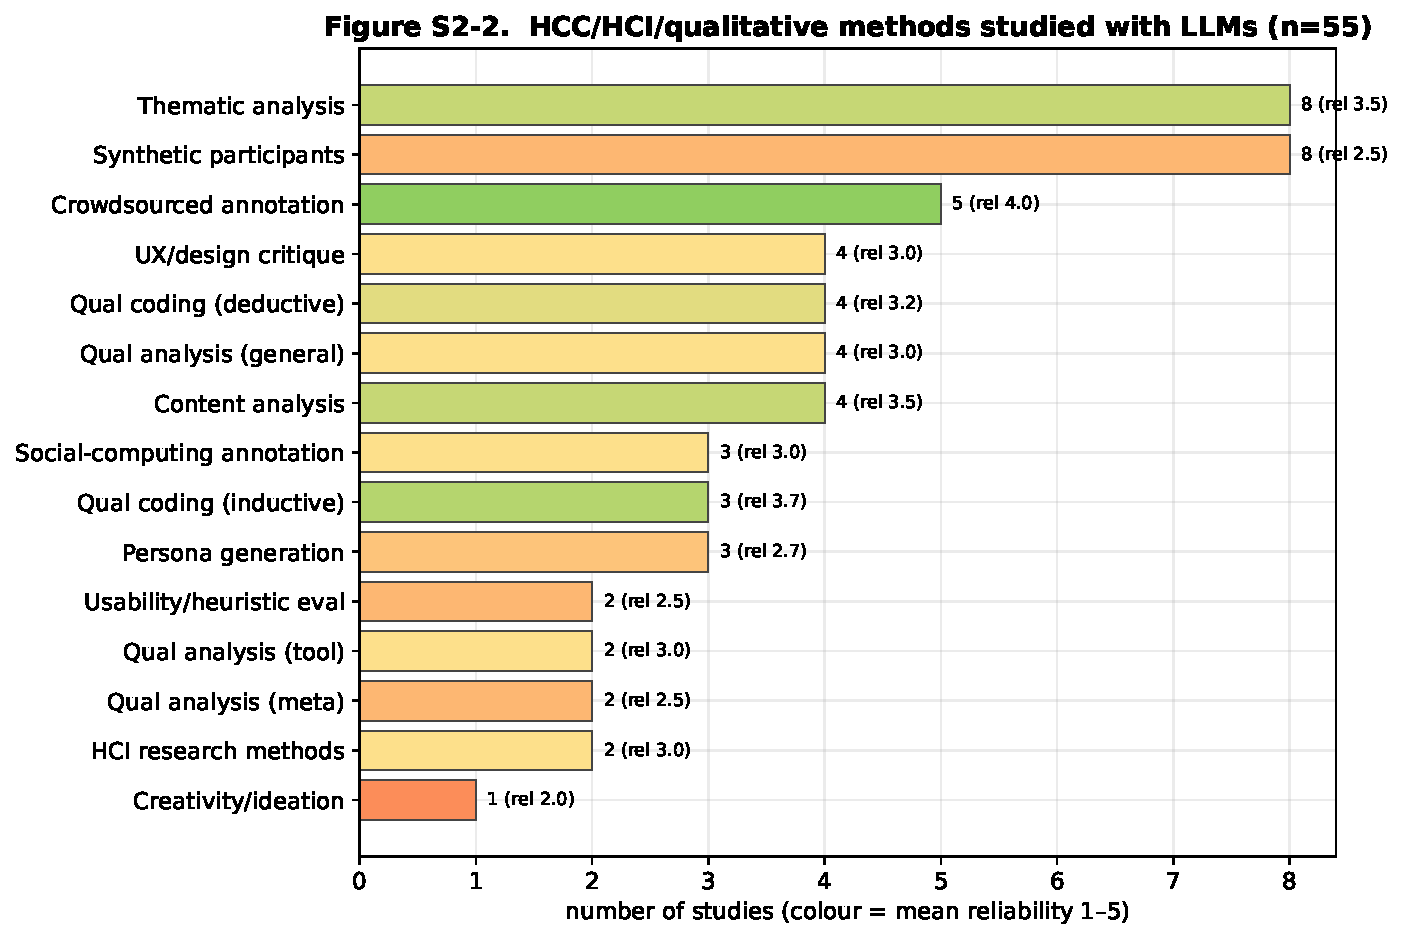
\includegraphics[width=\linewidth]{s2_fig02_methods}\caption{}\label{fig:s2methods}\end{subfigure}\hfill
\begin{subfigure}{0.46\linewidth}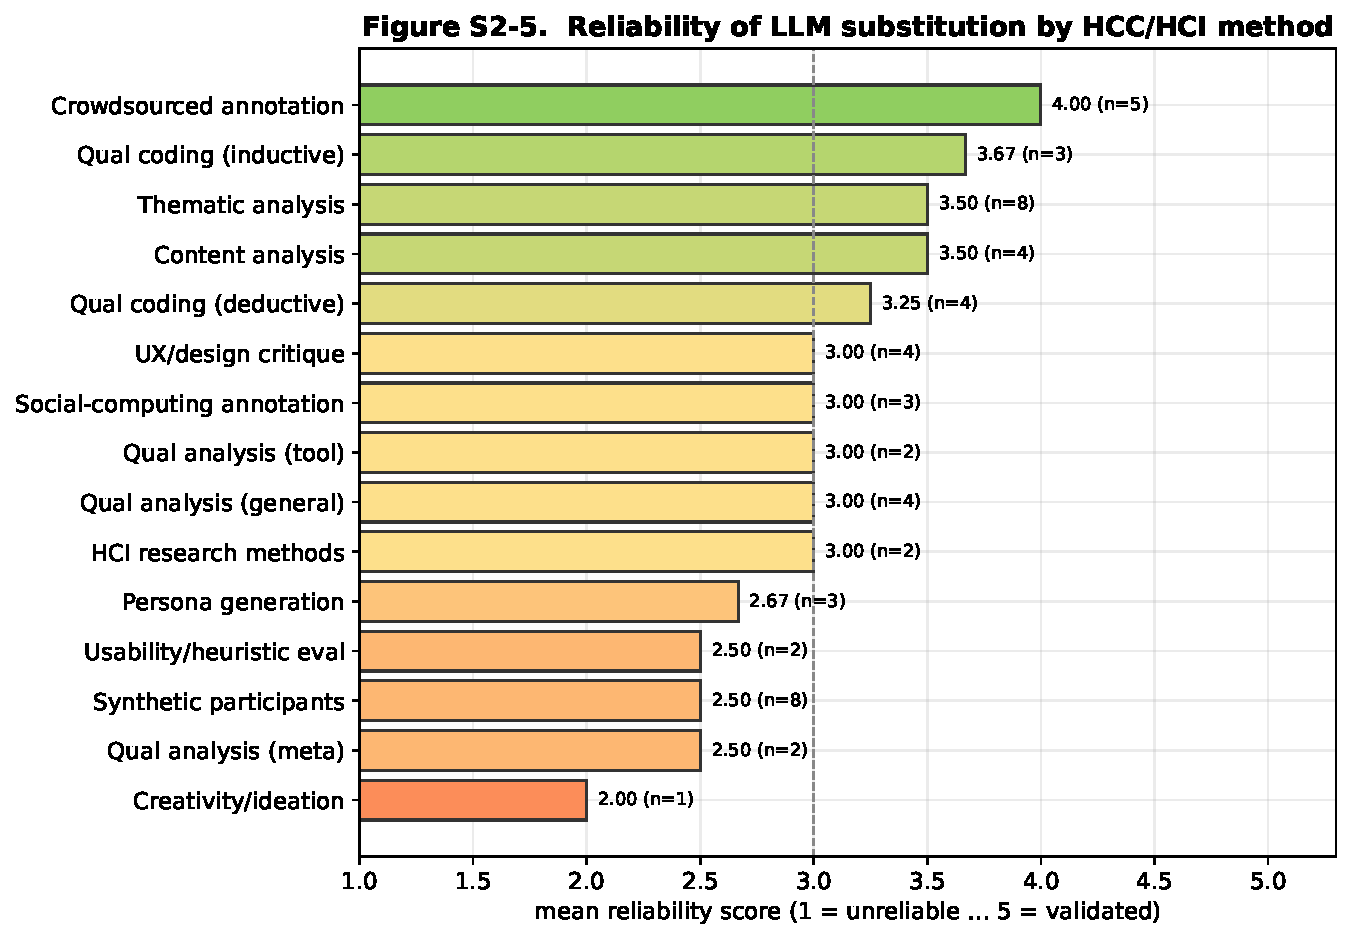
\includegraphics[width=\linewidth]{s2_fig05_reliability_by_method}\caption{}\label{fig:s2relmethod}\end{subfigure}
\caption{Study 1. (a) HCC/HCI/qualitative methods studied with LLMs (colour = mean reliability). (b) Mean reliability
of LLM substitution by method.}
\end{figure}

\begin{table}[t]\centering\small
\caption{Study 1 method-level decision table: study count, modal LLM role, mean reliability, and traffic-light
signal (\textsc{green} $\ge3.5$; \textsc{amber} 2.5-3.5; \textsc{red} $<2.5$).}
\label{tab:s2methods}
\begin{tabular}{@{}l r l c c@{}}
\toprule
Method & $n$ & Modal role & Mean rel. & Signal \\
\midrule
Crowdsourced annotation & 5 & replace & 4.00 & \cellcolor{g!55}\textsc{green} \\
Qual coding (inductive) & 3 & augment & 3.67 & \cellcolor{g!55}\textsc{green} \\
Content analysis & 4 & augment & 3.50 & \cellcolor{g!55}\textsc{green} \\
Thematic analysis & 8 & augment & 3.50 & \cellcolor{g!55}\textsc{green} \\
Qual coding (deductive) & 4 & augment & 3.25 & \cellcolor{a!60}\textsc{amber} \\
HCI research methods & 2 & augment & 3.00 & \cellcolor{a!60}\textsc{amber} \\
Qual analysis (general) & 4 & augment & 3.00 & \cellcolor{a!60}\textsc{amber} \\
Qual analysis (tool) & 2 & augment & 3.00 & \cellcolor{a!60}\textsc{amber} \\
Social-computing annotation & 3 & replace & 3.00 & \cellcolor{a!60}\textsc{amber} \\
UX/design critique & 4 & augment & 3.00 & \cellcolor{a!60}\textsc{amber} \\
Persona generation & 3 & augment & 2.67 & \cellcolor{a!60}\textsc{amber} \\
Qual analysis (meta) & 2 & augment & 2.50 & \cellcolor{a!60}\textsc{amber} \\
Synthetic participants & 8 & simulate & 2.50 & \cellcolor{a!60}\textsc{amber} \\
Usability/heuristic eval & 2 & replace & 2.50 & \cellcolor{a!60}\textsc{amber} \\
Creativity/ideation & 1 & augment & 2.00 & \cellcolor{r!55}\textsc{red} \\
\bottomrule
\end{tabular}
\end{table}

\subsection{RQ1.2: Augment, replace, or simulate?}
HCC overwhelmingly positions LLMs to \emph{augment} humans, not replace them: \STaugment{} of \STN{} studies frame
the LLM as a collaborator/assistant, versus \STreplace{} as a replacement and \STsimulate{} as a human simulator
(Figure~\ref{fig:s2rolestance}a). This is not merely rhetorical caution; it tracks reliability
(Figure~\ref{fig:s2verdictrole}): augmentation studies skew reliable, whereas \emph{replacement} is validated only
for objective annotation and \emph{simulation} of participants is the least reliable role
(mean reliability augment \STrelaugment{} vs.\ replace \STrelreplace{} vs.\ simulate \STrelsim{}). The replacement
mean is buoyed by objective crowd-annotation; remove it and replacement of \emph{interpretive} human input is
firmly amber/red. The canonical HCC workflow that emerges is human-in-the-loop: LLM proposes, human vets and retains
interpretive authority \citep{gao2024collabcoder,meng2024chalet,dai2023llminloop}.

\begin{figure}[t]\centering
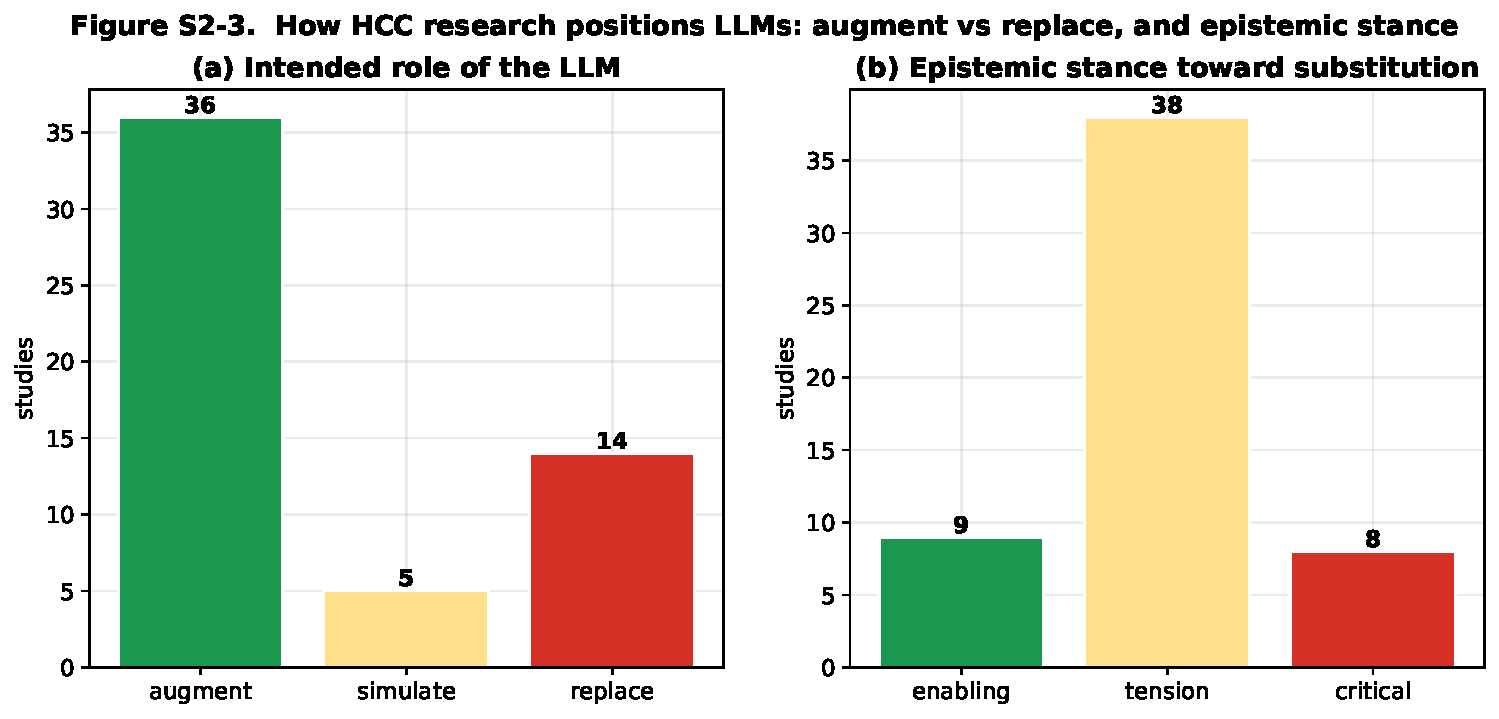
\includegraphics[width=0.95\linewidth]{s2_fig03_role_stance}
\caption{Study 1. (a) Intended LLM role across the HCC corpus; augmentation dominates. (b) Epistemic stance toward
substitution; \emph{tension} dominates.}
\label{fig:s2rolestance}
\end{figure}

\begin{figure}[t]\centering
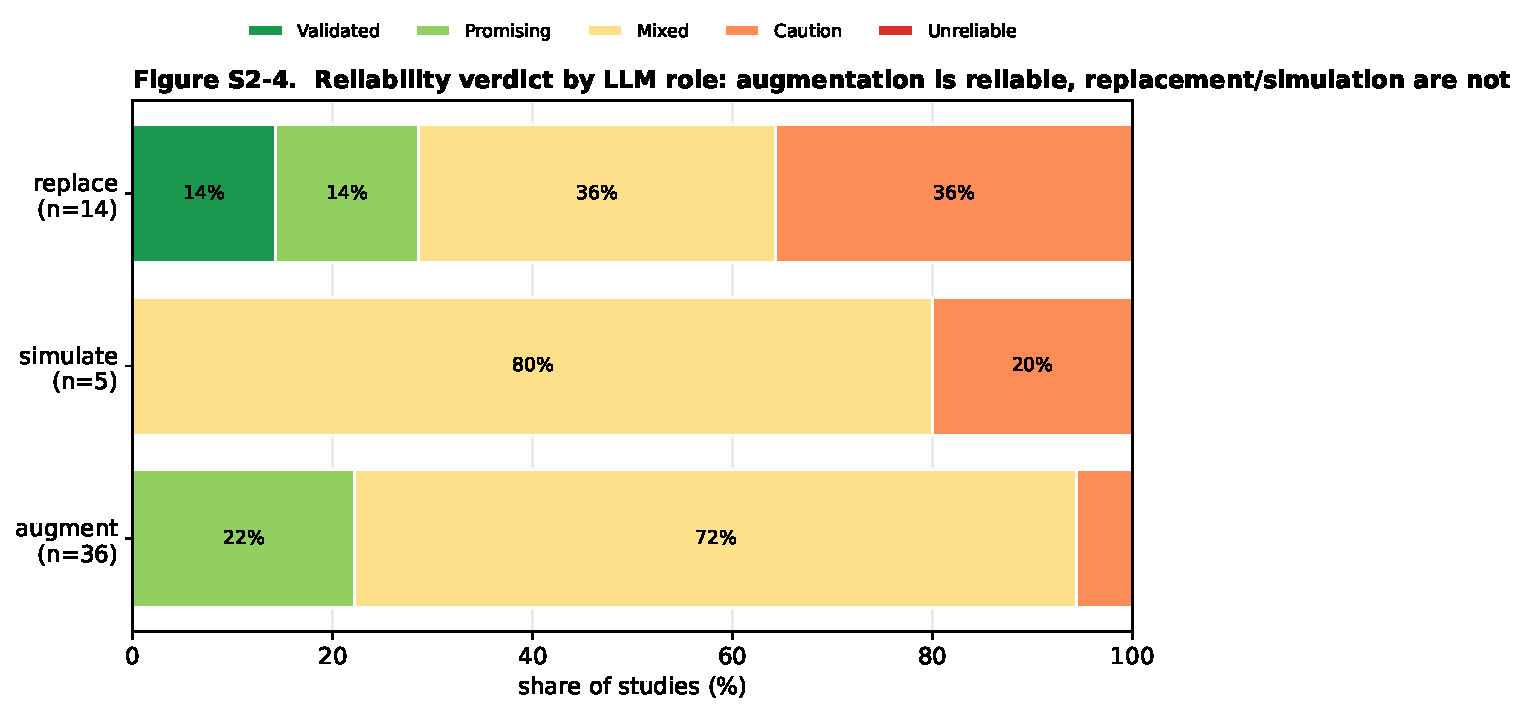
\includegraphics[width=0.8\linewidth]{s2_fig04_verdict_by_role}
\caption{Study 1. Reliability verdict by LLM role. Augmentation is reliable; replacement is reliable only for
objective annotation; participant/usability \emph{simulation} is the least reliable.}
\label{fig:s2verdictrole}
\end{figure}

\subsection{RQ1.3: Epistemic stance and the limits of substitution}
The dominant stance is \emph{tension} (\STtension/\STN), with \STcritical{} explicitly \emph{critical} and only
\STenabling{} unreservedly \emph{enabling} (Figure~\ref{fig:s2rolestance}b). Three threads recur.
\textbf{(i) Interpretation and reflexivity.} Qualitative scholars warn that LLMs perform surface-level extraction
well but cannot supply the situated, reflexive interpretation that gives qualitative findings their validity, and
that ``conditional trust'' in tool output risks hollowing out analytic rigor \citep{schroeder2025usestensions,
ngo2026chatqda,davison2024ethics,nguyentrung2025chatgptta}.
\textbf{(ii) Participants and identity.} Replacing human participants with LLMs \emph{flattens and misportrays}
demographic groups, positionality cannot be simulated \citep{wang2024flatten}, and LLM ``subgroups'' are often
caricatures \citep{cheng2023compost}; synthetic survey data distort variances and correlations
\citep{bisbee2023perils}, and an LLM is worth only a bounded number of real respondents \citep{huang2025surveyworth}.
HCI critiques accordingly recast synthetic users as ``objects of inquiry,'' not stand-ins \citep{salminen2025syntheticcritical,
haxvig2025personabias}.
\textbf{(iii) Expert design judgment.} GPT-4o overlaps only 21\% with expert-found usability issues and hallucinates
false positives \citep{guerino2025gpt4ousability}, and LLM UI critique trails expert designers
\citep{duan2024uicrit}, though synthetic heuristic evaluation can exceed \emph{novice} evaluators on issue recall
\citep{zhong2025synthheuristic}. Figure~\ref{fig:s2comm} shows coverage skews to HCI and computational social
science, with the augment-replace reliability gap visible across communities.

\begin{figure}[t]\centering
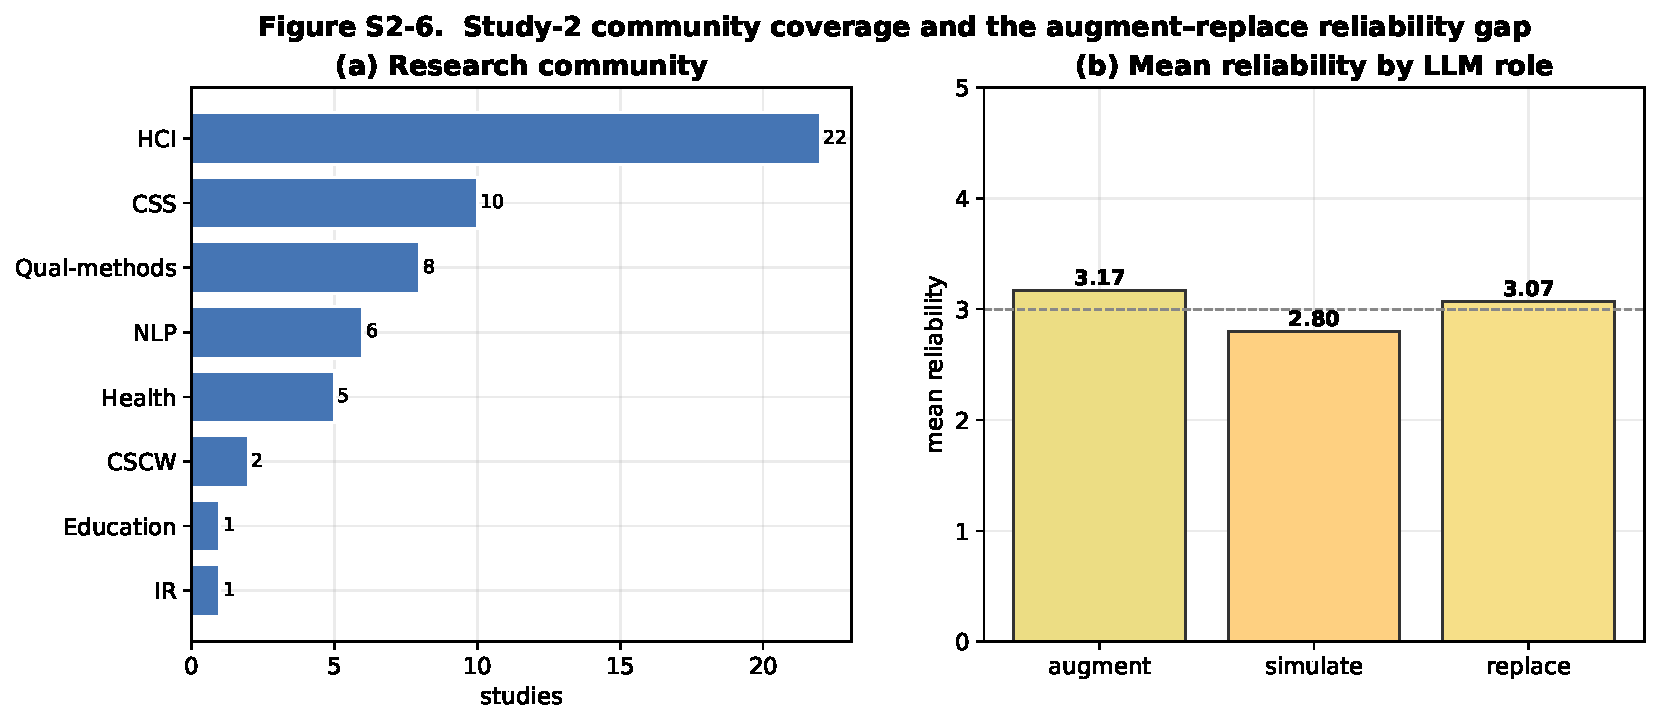
\includegraphics[width=0.95\linewidth]{s2_fig06_community_role}
\caption{Study 1. (a) Coverage by research community. (b) Mean reliability by LLM role, augmentation $>$
replacement $>$ simulation.}
\label{fig:s2comm}
\end{figure}

\subsection{Study 1 synthesis}
For HCC research, the evidence supports a clear, conditional posture.
\textbf{Validated to substitute:} objective crowd/data annotation (stance, topic, relevance, frames) where a human
ceiling is modest and verifiable.
\textbf{Reliable only as augmentation (human-in-the-loop):} deductive/inductive qualitative coding and thematic/
content analysis: LLMs accelerate breadth and first-pass coding, but humans must own interpretation, theme
development, and reflexive accounting.
\textbf{Unsafe to substitute:} simulating human participants, generating personas as stand-ins for real users, and
replacing expert usability/design judgment: these flatten identity, fabricate issues, and forfeit the situated
knowledge that defines human-centered inquiry. This posture both confirms the cross-domain objective/subjective prediction
\emph{within} HCC and exposes concrete gaps (\S\ref{sec:study2emp}) where HCC datasets with human labels have never
been formally tested with an LLM judge.

% =====================================================================
% =====================================================================
\section{Study 2: An empirical test on subjective social-computing annotation}\label{sec:study2emp}
% =====================================================================
The review establishes what the field \emph{believes} (augment, do not replace) but not whether that belief is
empirically warranted on the tasks HCC depends on. Study 2 supplies the missing evidence on the central case:
subjective social-computing annotation. We evaluate a panel of \STHRmodels{} open models (9B-754B, served via
\PROVIDER{} at temperature~0) as virtual annotators on \SOCndat{} datasets that ship human label distributions, the
constructs HCC and CSCW routinely label: \textbf{emotion} (GoEmotions, an authors-defined 4-way sentiment grouping),
binary \textbf{offensiveness} (SBIC), 3-way \textbf{hate speech} (HateXplain), and binary \textbf{irony} (MultiPICo,
a 2024 perspectivist corpus). The run comprised \SOCnjudg{} judgments with zero API errors and a 100\% parse rate.

\subsection{Method}
Each model labels every item under the same guidelines the human annotators received. We benchmark against the
\emph{human-human ceiling} (random-annotator-vs-majority accuracy with an annotator-bootstrap 95\% CI) and report
accuracy, Cohen's $\kappa$, macro-F1, a majority \textbf{jury} \citep{verga2024poll}, and a calibrated contamination
screen. Because subjective labels are not a single ``gold'' \citep{aroyo2015truth,plank2022humanlabel}, we also
report disagreement-aware metrics: panel accuracy stratified by item human-entropy, and the Jensen-Shannon
divergence between the panel and human label distributions. Dataset cards, prompts, and metric definitions are in
Appendices~\ref{app:protocol} to~\ref{app:robust}.

\subsection{The augment-not-replace consensus is empirically warranted}
On every subjective construct the open panel falls short of the human ceiling (Table~\ref{tab:socres}). Binary
offensiveness is the strongest case (\textbf{Promising}; best 0.86) yet still below its 0.91 ceiling; multi-way
emotion and 3-way hate are \textbf{Mixed} (best 0.61 / 0.66); and even where headline accuracy looks high, it
reflects base-rate learning rather than construct competence: on the recent irony corpus the best model reaches 0.82
accuracy but only $\kappa{=}0.40$. Chance-corrected agreement (Table~\ref{tab:socdis}) is modest throughout, exactly
the pattern the review's augment-not-replace consensus predicts.

\begin{table}[t]\centering\small
\caption{Study 2. Open panel vs the human-human ceiling on \SOCndat{} subjective social-computing datasets. Ceiling
= random-annotator-vs-majority accuracy; macro-F1 is the best model's chance-corrected score.}
\label{tab:socres}
\begin{tabular}{@{}l l c c c c l@{}}
\toprule
Dataset & Construct & Human & Best model & macro-F1 & Jury & Modal verdict \\
 & & ceiling & (acc) & (best) & (acc) & \\
\midrule
GoEmotions & emotion (4-way) & 0.78 & 0.61 (qwen3.6-27b) & 0.54 & 0.61 & \cellcolor{a!60}Mixed \\
SBIC & offensive (binary) & 0.91 & 0.86 (glm-5.1) & 0.85 & 0.84 & \cellcolor{g!25}Promising \\
HateXplain & hate (3-way) & 0.83 & 0.66 (gemma-4-31b) & 0.64 & 0.62 & \cellcolor{a!60}Mixed \\
MultiPICo & irony (binary) & 0.82 & 0.82 (gemma-4-31b) & 0.70 & 0.83 & \cellcolor{g!25}Promising \\
\bottomrule
\end{tabular}
\end{table}

\subsection{The shortfall is largest where humans agree, and is not a label-noise artifact}
A natural worry is that judges look worse on high-disagreement items simply because the majority gold is noisier
there (a tautology). The judge-vs-ceiling \emph{gap} rules this out. Raw accuracy does fall on high-entropy items
($\SOCaccLowE$ low-entropy vs $\SOCaccHighE$ high-entropy), but the gap below the human ceiling is in fact
\emph{largest on the low-entropy items where humans most agree} ($\SOCgapLow$ vs $\SOCgapHigh$): on clear-consensus
social items, where there is a definite human answer, the panel still misses it by a wide margin. This is a genuine
substitution failure, not noise on ambiguous cases. The residual variance is item-level: in an item-level GLMM the
random-intercept SD across \emph{items} ($\mathrm{SD}_{\text{logit}}=\SOCitemSDlogit$) far exceeds that across
\emph{models} ($\mathrm{SD}_{\text{logit}}=\SOCmodelSDlogit$, on the same logit scale), and standardized model scale
contributes only modestly ($\mathrm{OR}_{/\mathrm{SD}}=\RTwosizeOR$); with four datasets we do not fit a
dataset-level model. Contamination does not explain the shortfall: the recent (2024) MultiPICo corpus, which the
low-recall judge has not memorized, is matched only at its low ceiling, so the limitation tracks human judgment, not
pretraining exposure (the verbatim screen is conservative, Appendix~\ref{app:robust}).

\begin{table}[t]\centering\small
\caption{Study 2 disagreement-aware results. Ceiling with annotator-bootstrap 95\% CI; best-model $\kappa$ and
macro-F1; panel accuracy on low- vs high-human-disagreement items; Jensen-Shannon panel-vs-human divergence. Judges
lose accuracy precisely as human disagreement rises.}
\label{tab:socdis}
\begin{tabular}{@{}l c c c c c c@{}}
\toprule
Dataset & Ceiling [95\% CI] & $\kappa$ & macro-F1 & acc$_{\downarrow H}$ & acc$_{\uparrow H}$ & JS \\
 & & (best) & (best) & low-disagr. & high-disagr. & \\
\midrule
GoEmotions & 0.78 [0.76,0.80] & 0.44 & 0.54 & 0.60 & 0.45 & 0.31 \\
SBIC & 0.91 [0.89,0.92] & 0.71 & 0.85 & 0.86 & 0.61 & 0.10 \\
HateXplain & 0.83 [0.82,0.85] & 0.49 & 0.64 & 0.66 & 0.48 & 0.27 \\
MultiPICo & 0.82 [0.81,0.83] & 0.40 & 0.70 & 0.80 & 0.63 & 0.09 \\
\bottomrule
\end{tabular}
\end{table}

\paragraph{What this means for HCC.} The model that simply predicts the majority looks accurate but erases the
minority readings that perspectivist annotation is designed to preserve, which is precisely the flattening HCC warns
against \citep{wang2024flatten,fricker2007epistemic}. Empirically, then, the field's instinct is right: for
subjective social annotation an LLM is a useful first-pass assistant but not a replacement for the human annotators
whose disagreement \emph{is} the signal.
% =====================================================================
\section{Discussion}
% =====================================================================
\subsection{Review and experiment agree}
The review and the experiment tell one story. The field positions LLMs to \emph{augment} rather than replace humans,
with reliability ordered augment $>$ replace $>$ simulate; the experiment shows why that ordering is correct for the
field's central labeling case. On subjective social-computing constructs, open judges do not reach the human-human
ceiling, and their errors are not random: they concentrate on the items where humans themselves disagree. The
binding constraint is therefore not model capability but the contested human reference, which is exactly the
property that makes these constructs ``human-centered'' in the first place.

\subsection{Connections to HCI and measurement scholarship}
Three HCI conversations are sharpened by this evidence. \textbf{(1) There is no single ground truth.} CSCW and HCI
have long argued that inter-rater reliability is a negotiated practice, not a natural fact
\citep{mcdonald2019reliability}, and NLP has reframed annotator disagreement as signal \citep{aroyo2015truth,
plank2022humanlabel}; benchmarking against the human ceiling makes the judges' ``failures'' legible as properties of
the construct, not fixable model deficits. \textbf{(2) Interpretation is not labeling.} Reflexive thematic analysis
treats coding as situated interpretation \citep{braun2006thematic}, and qualitative scholars warn that ``conditional
trust'' in LLM output hollows out rigor \citep{schroeder2025usestensions,davison2024ethics}; the augment-not-replace
consensus and the empirical shortfall are two views of the same boundary. \textbf{(3) Participants are not
simulable.} The ``silicon sample'' program \citep{argyle2023outofone} meets a growing critique that simulated
participants flatten identity \citep{wang2024flatten,cheng2023compost,bisbee2023perils,salminen2025syntheticcritical};
our finding that judges default to majority readings and lose the minority signal is that flattening at the level of
a single subjective label, a representational harm a single accuracy number conceals \citep{fricker2007epistemic,
birhane2022values}.

\subsection{A critical assessment for the field}
We name two risks the community should track, marking what our data support and what extends prior critique.
\textbf{False closure (data-grounded).} Reporting one accuracy against a majority gold imposes consensus where the
data shows disagreement; our irony case (0.82 accuracy at $\kappa{=}0.40$) shows how a headline number masks
base-rate learning. \textbf{Monoculture and deskilling (conjecture).} Cheap labeling invites substituting LLM
judgment for the human annotation and reflexive interpretation that train researchers; combined with the documented
convergence of judges toward crowd rather than expert consensus \citep{bavaresco2024judgebench} and the way
technical framings abstract away the social context of measurement \citep{selbst2019abstraction,suchman2007humanmachine},
this could erode the field's interpretive capacity. We offer it as a hypothesis, not a finding.

\subsection{A decision framework for HCC}
\begin{itemize}[leftmargin=1.4em,itemsep=2pt]
\item \textbf{Automate (with light audit):} objective annotation of user-generated content (stance, topic, frames)
where the human ceiling is high and verifiable \citep{gilardi2023chatgpt,tornberg2023political}.
\item \textbf{Augment, human-in-the-loop:} subjective coding and thematic/content analysis: use the LLM for
first-pass coding, breadth, and disagreement surfacing, but keep human interpretive authority, calibrate on a
labeled subset, and report chance-corrected agreement against human coders \citep{gao2024collabcoder,dai2023llminloop}.
\item \textbf{Keep humans (do not substitute):} simulating participants or personas, and replacing expert
usability/design judgment, which flatten identity and forfeit situated knowledge
\citep{wang2024flatten,guerino2025gpt4ousability,salminen2025syntheticcritical}.
\end{itemize}
Practically, any HCC study reporting LLM-assisted analysis should state the LLM's \emph{role}, benchmark against a
\emph{human-human} baseline at the right granularity, report chance-corrected and disagreement-aware metrics with
uncertainty, evaluate on post-cutoff data where possible, and treat minority annotator readings as signal rather
than noise.
% =====================================================================
\section{Limitations}
% =====================================================================
The \emph{human} validation here is inherited from prior work, not added by us: Study 2's ground truth is each
dataset's own human annotators (3 to 8 per item), and the review codes each study against the human baselines those
studies report. The review verdict is our interpretation (only a minority of studies report an extractable numeric
agreement value); we report an independent re-coding as a reproducibility check (verdict Krippendorff
$\alpha=\IRRstwoV$, role $\alpha=\IRRstwoRole$, the more interpretive stance $\alpha=\IRRstwoStance$;
Appendix~\ref{app:irr}), which is LLM-assisted and therefore measures rubric reproducibility; we treat stance claims
as indicative. All references were web-verified. By design we evaluate \emph{open} models (the reproducible choice
for most HCC labs) at temperature~0 across \SOCndat{} subjective datasets; interpretive qualitative coding,
participant simulation, and design judgment are characterized by the review rather than tested empirically here.
Findings reflect models available through mid-2026.
\section{Ethics and reproducibility}
% =====================================================================
\textbf{Ethics.} The review analyzes published research, not human subjects, and Study 3 reuses already-public,
de-identified datasets under their licenses; this work was therefore not human-subjects research requiring IRB
review, and we sought an exemption determination consistent with our institution's policy. Two datasets (HateXplain,
SBIC) contain hateful or identity-attacking text, which we process only to measure moderation reliability and never
reproduce; to avoid redistributing harmful or personally-identifiable content we release only item-level labels and
aggregate statistics, never the raw texts. A deeper ethical point bears on our own method: by treating the
\emph{majority} human label as ``ground truth'' for the ceiling, we risk encoding majority-group bias and erasing
minority readings, exactly the harm we warn against. We mitigate this by (i) reporting the full disagreement (soft
labels, entropy) rather than only the majority, (ii) checking, where annotator demographics exist (MultiPICo), that
the panel does not agree disproportionately with one subgroup (gap $=\MPCgenderGap$; Appendix~\ref{app:robust}), and
(iii) recommending disagreement-aware evaluation in our guidance; we note the other corpora lack annotator
demographics, so this check is partial. The contamination probe is reported precisely so ``validated'' verdicts are
not silently inflated by pretraining exposure. The work is dual-use only in the benign sense that better-calibrated
LLM judges reduce the risk of unaccountable automated moderation; our central finding (that LLM judges should not replace humans on subjective social annotation) is itself a guard against premature deployment.
\textbf{Reproducibility.} Every number in this paper regenerates from released code: the OpenAlex, Semantic Scholar,
and web search logs; the coded corpus; the figure and table generators; the Study-2 judging/scoring/contamination/mixed-effects harness, all keyed to documented model identifiers served through
\PROVIDER{} at temperature~$0$ with idempotent, resumable checkpoints. The auto-generated statistics macros
mean the manuscript cannot drift from the data. Repository: \REPO{}.

% =====================================================================
% =====================================================================
\section{Conclusion}
% =====================================================================
Human-Centered Computing is right to position LLMs as assistants rather than replacements for human input. Across
\STN{} reviewed studies and a \SOCnjudg{}-judgment experiment on subjective social-computing annotation, the
evidence converges: open LLM judges do not reach the human-human agreement ceiling on contested constructs, and
their errors concentrate on exactly the items where humans disagree, which is the signal HCC cares about. The field
should treat an LLM judge as a measured instrument, reported against a human-human baseline with chance-corrected,
disagreement-aware metrics, used to augment and accelerate human interpretation rather than to stand in for the
humans whose disagreement constitutes the phenomenon under study.

\bibliographystyle{ACM-Reference-Format}
\bibliography{references}
\appendix
\section{Review protocol and reliability rubric}\label{app:protocol}
% =====================================================================
\paragraph{Identification.} The review follows PRISMA~2020. The primary bibliographic source is the
\textbf{OpenAlex} API; we cross-check with the \textbf{Semantic Scholar} Graph API and a structured
\textbf{web ``deep-research''} arm. The review used a
25-query HCC/HCI/qualitative concept-block protocol (the same query strings were issued against every source so the
arms are comparable). Concept blocks combine an LLM term (``LLM'', ``large language model'', ``GPT-4'', ``ChatGPT'',
``Gemini''), an evaluation/agreement term (``LLM-as-a-judge'', ``automatic evaluation'', ``annotation'', ``inter-annotator
agreement'', ``human evaluation''), and an HCC method term (``qualitative coding'', ``thematic analysis'',
``content analysis'', ``crowdsourcing'', ``participant simulation'', ``persona'', ``usability evaluation'', ``design
critique''). Records were deduplicated by DOI and normalized title.

\paragraph{Screening and eligibility.} \emph{Inclusion:} peer-reviewed or preprint studies that empirically compare
LLM judgments to human judgments on the same items and report (or allow computing) an agreement statistic.
\emph{Exclusion:} non-empirical position papers, studies with no human baseline, studies that use LLMs only to
generate (not judge) content, and off-topic retrievals. Title/abstract screening was followed by full-text
eligibility assessment; per-stage counts appear in the PRISMA flow figure (Figure~\ref{fig:s2prisma}).

\paragraph{Reliability verdict (five-level rubric).} Each study is coded against the \emph{human-human agreement
ceiling} for its task:
\begin{itemize}[leftmargin=1.4em,itemsep=1pt]
\item \textbf{1 Validated:} LLM-human agreement is at or above the human-human ceiling (substitution is empirically
justified).
\item \textbf{2 Promising:} agreement approaches the ceiling under specific, reported conditions (model, prompt,
aggregation); conditional substitution.
\item \textbf{3 Mixed:} results are task- or setup-dependent and inconsistent across studies.
\item \textbf{4 Caution:} agreement is consistently and materially below the ceiling.
\item \textbf{5 Unreliable:} agreement is near chance or dominated by bias (position, verbosity, self-preference).
\end{itemize}
We report a reliability score $=6-\text{verdict}$ and synthesize within metric families (e.g.\ Cohen's $\kappa$,
Krippendorff's $\alpha$, Spearman $\rho$, accuracy) rather than pooling incommensurable effect sizes. The full coded corpus (Appendix~\ref{app:s2}) is released for re-coding.

% =====================================================================
\section{Study 3: datasets, judging prompts, and metrics}\label{app:s3detail}
% =====================================================================
\paragraph{Datasets.} Study 2 uses \SOCndat{} subjective social-computing datasets (Table~\ref{tab:cardssoc}); each
is sampled to $n{=}500$ items with a clear majority label (ties dropped), using the per-item annotator distributions
to compute the human ceiling. MultiPICo (2024) is a recent corpus that serves as a post-cutoff condition.

\begin{table}[h]\centering\small
\caption{Study 2 dataset cards. Ceiling $=$ random-annotator-vs-majority accuracy.}
\label{tab:cardssoc}
\begin{tabular}{@{}l l l c c@{}}
\toprule
Dataset & Task & Source & Annot./item & Ceiling \\
\midrule
GoEmotions & sentiment (4-way, authors' grouping) & Reddit (Google) & ${\sim}3$-$5$ & 0.78 \\
SBIC & offensiveness (binary) & Social Bias Frames & ${\sim}3$ & 0.91 \\
HateXplain & hate speech (3-way) & Twitter/Gab & $3$ & 0.83 \\
MultiPICo & irony (binary) & Reddit/Twitter (2024) & $3$-$8$ & 0.82 \\
\bottomrule
\end{tabular}

\end{table}

\paragraph{Judging prompts.} Each model labels every item as a virtual annotator, returning a JSON label on the final
line (parsed with a surface-form-to-code map):
\begin{quote}\small\ttfamily
Emotion: Comment: \{text\} / Overall sentiment: POSITIVE, NEGATIVE, AMBIGUOUS, or NEUTRAL. -> \{"label": ...\}\\[2pt]
Offensive: Post: \{text\} / Is this post offensive (including potentially offensive)? -> \{"label": "offensive"|"not offensive"\}\\[2pt]
Hate: Post: \{text\} / HATE SPEECH (identity-targeted), OFFENSIVE (not group-targeted), or NORMAL. -> \{"label": ...\}\\[2pt]
Irony: \{post+reply\} / Is the REPLY ironic/sarcastic, or not ironic? -> \{"label": "ironic"|"not ironic"\}
\end{quote}

\paragraph{Metrics.} Let an item have $A$ human annotations with majority label $y^\star$. \textbf{Human ceiling} is
the random-annotator-vs-majority accuracy averaged over items, with an annotator-bootstrap 95\% CI. \textbf{Accuracy},
\textbf{Cohen's $\kappa$}, and \textbf{macro-F1} are against $y^\star$; the \textbf{jury} is the per-item panel
majority \citep{verga2024poll}; \textbf{95\% CIs} are nonparametric bootstrap (1000 item resamples). A
\textbf{contamination screen} (one-third-prefix verbatim reproduction) is reported as a conservative check; a
clean-control (Appendix~\ref{app:robust}) shows it false-positives on high-recall models, so we rely on the recent
MultiPICo post-cutoff condition. The run recorded \emph{zero} API errors and a 100\% answer-parse rate across all
\SOCnjudg{} judgments.

\paragraph{Inferential model.} We model each judgment's correctness with an item-level Bayesian logistic GLMM with
random intercepts for item and model, reporting variance components on a common logit scale (item
$\mathrm{SD}_{\text{logit}}=\SOCitemSDlogit$, model $\SOCmodelSDlogit$). With four datasets we do not fit a
dataset-level model. We bin items by human entropy and report the judge-vs-ceiling \emph{gap} per bin to show the
shortfall is not a label-noise artifact (the gap is largest where humans most agree, see the main text).

% =====================================================================
\section{Inter-coder reliability}\label{app:irr}
% =====================================================================
Because the reliability verdict and the role/stance codes embed judgement, we re-coded a held-out random sample of
each corpus with two \emph{independent} coders who saw only the per-study summaries and the rubric (no original
codes, no other context). For the review ($n{=}\IRRstwoN$, a 30\% sample) the reliability verdict reproduced at
Krippendorff $\alpha=\IRRstwoV$, the augment/replace/simulate role at $\alpha=\IRRstwoRole$, and the epistemic stance
at $\alpha=\IRRstwoStance$ (the least reliable code). \emph{Caveat:} the re-coders are
LLM-assisted, like the primary pipeline, so these figures measure rubric \emph{reproducibility} under independent
application, not human inter-rater agreement; the moderate stance $\alpha$ is why we treat stance-based claims as
indicative.

% =====================================================================
\section{Robustness and validity checks}\label{app:robust}
% =====================================================================
\textbf{Prompt robustness.} We re-ran a robustness subset (three models, $n{=}120$ per cell) under
three semantically equivalent prompt paraphrases per task. \emph{Accuracy} is fairly prompt-stable (mean SD across
paraphrases $=\PRmeanSD$), but the discrete five-level \emph{verdict} is exactly stable in only \PRstable{}/\PRtotal{}
cells: most instability is a one-level flip for cells sitting near a band boundary, and the smaller model is the most
sensitive (worst-case acc SD $\PRmaxSD$), the larger models the least. We therefore report verdicts as robust to
\emph{within one level} rather than exact, and flag small-model verdicts on subjective tasks as prompt-sensitive.
\textbf{Contamination clean control.} We ran the verbatim-recall probe on freshly authored, post-cutoff sentences
that no model can have seen. The result is a cautionary one: the high-recall model still scores $\CCmaxOverlap$ mean
overlap (\CCflag) on this guaranteed-clean text, i.e.\ it confabulates plausible continuations regardless of
memorization, while the low-recall model scores LOW. The probe thus has a high false-positive rate for high-recall
models and \emph{cannot} be read as a reliable leakage test; the uniform MEDIUM tiers in Table~\ref{tab:socres} are
largely an artifact of generative fluency. We retain the probe only as a conservative, low-recall-model signal and
base our substantive claims on the disagreement analysis instead.
\textbf{Annotator-subgroup check.} On MultiPICo (which carries annotator demographics), the panel's agreement with
the female- vs male-annotator majority differs by only \MPCgenderGap, i.e.\ we did not detect a large majority-group
bias in this corpus, though demographic metadata is sparse and this check is limited.
\textbf{Ceiling vs annotator count.} The random-annotator-vs-majority ceiling depends on how many annotators an item
has: subsampling ChaosNLI-SNLI (${\sim}100$ annotators) to $A{=}3$ raises its estimated ceiling from
\RTwoablCeilFull{} to \RTwoablCeilThree{} (fewer annotators yield more unanimous majorities). We therefore compute
each dataset's ceiling at its \emph{native} annotator count and caution that ceilings are not directly comparable
across datasets with very different $A$; the disagreement-aware analyses (entropy, $\kappa$) do not depend on this
estimator.

% =====================================================================
\section{Study 2 corpus}\label{app:s2}
% =====================================================================
\footnotesize
\begin{longtable}{@{}l l l l c l@{}}
\caption{Study 2 corpus (55 studies): HCC/HCI/qualitative methods using LLMs vs human input.}\label{tab:study2full}\\
\toprule
Study & Method & Role & Community & Agree & Verdict \\
\midrule
\endfirsthead
\toprule Study & Method & Role & Community & Agree & Verdict \\ \midrule \endhead
Chew et al. (2023) & Content analysis & augment & CSS & -- & Promising \\
Leas et al. (2023) & Content analysis & augment & Health & -- & Mixed \\
Long et al. (2024) & Content analysis & augment & Education & -- & Mixed \\
Dunivin (2025) & Content analysis & augment & CSS & -- & Promising \\
Anderson et al. (2024) & Creativity/ideation & augment & HCI & -- & Caution \\
Gilardi et al. (2023) & Crowdsourced annotation & replace & CSS & -- & Validated \\
Tornberg (2023) & Crowdsourced annotation & replace & CSS & -- & Validated \\
Kuzman et al. (2023) & Crowdsourced annotation & replace & NLP & -- & Mixed \\
Li et al. (2023) & Crowdsourced annotation & augment & NLP & -- & Promising \\
Ostyakova et al. (2023) & Crowdsourced annotation & replace & NLP & -- & Mixed \\
Tabone \& de Winter (2023) & HCI research methods & augment & HCI & -- & Mixed \\
Aubin Le Quere et al. (2024) & HCI research methods & augment & HCI & -- & Mixed \\
Salminen et al. (2024) & Persona generation & augment & HCI & -- & Mixed \\
Jung et al. (2025) & Persona generation & augment & HCI & -- & Mixed \\
Haxvig et al. (2025) & Persona generation & replace & HCI & -- & Caution \\
Zhang et al. (2023) & Qual analysis (general) & augment & Qual-methods & -- & Mixed \\
Wachinger et al. (2024) & Qual analysis (general) & augment & Health & -- & Mixed \\
Li et al. (2024) & Qual analysis (general) & augment & Health & 0.40 & Mixed \\
Mehta et al. (2025) & Qual analysis (general) & augment & Qual-methods & -- & Mixed \\
Davison et al. (2024) & Qual analysis (meta) & augment & CSS & -- & Caution \\
Schroeder et al. (2025) & Qual analysis (meta) & augment & HCI & -- & Mixed \\
Zhang et al. (2024) & Qual analysis (tool) & augment & HCI & -- & Mixed \\
Meng et al. (2024) & Qual analysis (tool) & augment & HCI & -- & Mixed \\
Xiao et al. (2023) & Qual coding (deductive) & augment & HCI & -- & Promising \\
Savelka et al. (2023) & Qual coding (deductive) & augment & NLP & -- & Mixed \\
Zhang et al. (2025) & Qual coding (deductive) & augment & Qual-methods & 0.46 & Mixed \\
authors (2025) & Qual coding (deductive) & augment & Qual-methods & 0.46 & Mixed \\
Gao et al. (2024) & Qual coding (inductive) & augment & HCI & -- & Promising \\
Dunivin (2024) & Qual coding (inductive) & replace & Qual-methods & -- & Promising \\
Ngo et al. (2026) & Qual coding (inductive) & augment & HCI & -- & Mixed \\
Wu et al. (2023) & Social-computing annotation & replace & CSCW & -- & Mixed \\
Zhu et al. (2023) & Social-computing annotation & replace & CSCW & -- & Mixed \\
Rajashekar et al. (2024) & Social-computing annotation & augment & HCI & -- & Mixed \\
Argyle et al. (2023) & Synthetic participants & simulate & CSS & -- & Mixed \\
Bisbee et al. (2023) & Synthetic participants & replace & CSS & -- & Caution \\
Cheng et al. (2023) & Synthetic participants & simulate & NLP & -- & Caution \\
Wang et al. (2024) & Synthetic participants & replace & HCI & -- & Caution \\
Bail (2024) & Synthetic participants & simulate & CSS & -- & Mixed \\
Abbasiantaeb et al. (2024) & Synthetic participants & simulate & IR & -- & Mixed \\
Huang et al. (2025) & Synthetic participants & simulate & CSS & -- & Mixed \\
Salminen et al. (2025) & Synthetic participants & replace & HCI & -- & Caution \\
De Paoli (2023) & Thematic analysis & augment & CSS & -- & Mixed \\
Dai et al. (2023) & Thematic analysis & augment & NLP & -- & Promising \\
Prescott et al. (2024) & Thematic analysis & augment & Health & -- & Mixed \\
Nguyen-Trung (2025) & Thematic analysis & augment & Qual-methods & -- & Mixed \\
Jain et al. (2025) & Thematic analysis & replace & Qual-methods & 0.91 & Promising \\
Castellanos et al. (2025) & Thematic analysis & augment & Health & 0.80 & Promising \\
Sharma et al. (2025) & Thematic analysis & augment & HCI & -- & Promising \\
Wen et al. (2025) & Thematic analysis & augment & Qual-methods & -- & Mixed \\
Kocaballi (2023) & UX/design critique & augment & HCI & -- & Mixed \\
Duan et al. (2024) & UX/design critique & augment & HCI & -- & Mixed \\
Duan et al. (2024) & UX/design critique & augment & HCI & -- & Mixed \\
Duan et al. (2024) & UX/design critique & augment & HCI & -- & Mixed \\
Guerino et al. (2025) & Usability/heuristic eval & replace & HCI & 0.21 & Caution \\
Zhong et al. (2025) & Usability/heuristic eval & replace & HCI & 0.75 & Mixed \\
\bottomrule
\end{longtable}

\end{document}
